\chapter{Exchange Between Cells and Their
Environment}\label{exchange-between-cells-and-their-environment}

\section{Diffusion}\label{diffusion}

\href{https://en.wikipedia.org/wiki/Diffusion}{Diffusion} is the net
movement of molecules or atoms from a region of high concentration (or
high chemical potential) to a region of low concentration (or low
chemical potential) as a result of random motion of the molecules or
atoms. The word diffusion derives from the Latin word, diffundere, which
means ``to spread way out''.

Diffusion is driven by a gradient in chemical potential of the diffusing
species. A gradient is the change in the value of a quantity
e.g.~concentration, pressure, or temperature with the change in another
variable, usually distance. A change in concentration over a distance is
called a concentration gradient, a change in pressure over a distance is
called a pressure gradient, and a change in temperature over a distance
is a called a temperature gradient.

A distinguishing feature of diffusion is that it depends on particle
random walk, and results in mixing or mass transport without requiring
directed bulk motion.

\subsection{Diffusion in air}\label{diffusion-in-air}

\subsection{Experimental procedures}\label{experimental-procedures}

\begin{enumerate}
\def\labelenumi{\arabic{enumi}.}
\tightlist
\item
  The instructor will open a bottle containing a fragrant substance.
\item
  Raise your hand when you smell the odor.
\end{enumerate}

\subsection{Diffusion in water}\label{diffusion-in-water}

\subsection{Experimental
procedures}\label{experimental-procedures-1}

\begin{enumerate}
\def\labelenumi{\arabic{enumi}.}
\tightlist
\item
  Add 10 mL of water to a plastic test tube.
\item
  Drop a crystal of purple KMnO\textsubscript{4} (potassium
  permanganate) into it.
\item
  Put the tube in a test tube rack and place it where it will not be
  disturbed for the remainder of the lab period
\item
  From time to time, observe the how the KMnO\textsubscript{4} diffuses
  through the water.
\end{enumerate}

\subsection{Diffusion in a solid}\label{diffusion-in-a-solid}

\subsection{Experimental
procedures}\label{experimental-procedures-2}

\begin{enumerate}
\def\labelenumi{\arabic{enumi}.}
\tightlist
\item
  Place a few crystals of KMnO\textsubscript{4} onto a Petri dish with
  agarose gel.
\item
  Place a few crystals of malachite green about 2 centimeters from the
  potassium permanganate crystal.
\item
  Place a few specks of carmine red about 2 cm from each of the other crystals.
\item
  Note the rate of diffusion.
\item
  Find the molecular weights of each compound from
  \href{https://www.wikipedia.org}{Wikipedia}.
\end{enumerate}

\subsection{Diffusion Through a Selectively Permeable
Membrane}\label{diffusion-through-a-selectively-permeable-membrane}

A selectively permeable membrane is a type of biological or synthetic, polymeric membrane that will allow certain molecules or ions to pass through it by diffusion—or in the case of bioloigcal membranes (e.g. the cell membrane) by more specialized processes such as facilitated diffusion and active transport. In this experiment we will use a dialysis or \href{https://en.wikipedia.org/wiki/Semipermeable_membrane}{semipermeable membrane}–a selectively permeable membrane that allows particles below a certain size through but excludes any particles that are larger. 

\subsection{Experimental procedures}\label{experimental-procedures-14}

\begin{enumerate}
\def\labelenumi{\arabic{enumi}.}
\tightlist
\item
  Fill a 500-ml beaker with 300 ml of water.
\item
  Get a \textasciitilde{} 10 cm long piece of dialysis tubing and
  submerge it for \textasciitilde{} 10 seconds in the water.
\item
  Remove the dialysis tubing and clamp one end with the yellow clamp.
\item
  Rub the other end between the tips of your thumb and index fingers to
  open the dialysis membrane.
\item
  Get the starch solution and shake it well.
\item
  Fill the dialysis tubing with \textasciitilde{} 10 ml of starch
  solution.
\item
  Clamp off the open end.
\item
  Rinse with tap water.
\item
  Add iodine solution to the beaker with water until the solution
  becomes dark orange.
\item
  Add the dialysis tube containing the starch to the beaker and submerge
  completely in the water.
\item
  After about 15 minutes, observe the bag and surrounding liquid for any
  color change.
\item
  When starch molecules touch iodine, a blue or purplish color appears.
\item
  Start setting up Experiment 3 while you wait.
\end{enumerate}

\begin{figure}

{\centering 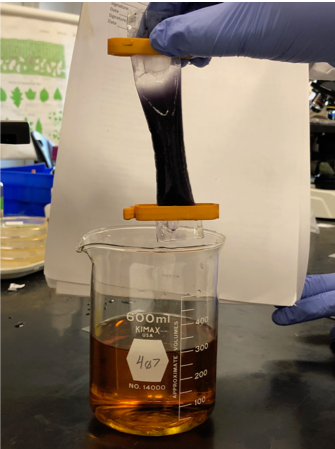
\includegraphics[width=0.7\linewidth]{./figures/exchange/Dialysis}

}

\caption{Result of the dialysis experiment.}\label{fig:dialysis}
\end{figure}

\section{Brownian motion}\label{brownian-motion}

\href{https://en.wikipedia.org/wiki/Brownian_motion}{Brownian motion} is
the random motion of particles suspended in a fluid (a liquid or a gas)
resulting from their collision with the fast-moving molecules in the
fluid. This motion is named after
\href{https://en.wikipedia.org/wiki/Robert_Brown_(botanist,_born_1773)}{Robert
Brown} (botanist, born 1773). In 1827, while looking through a
microscope at particles trapped in cavities inside pollen grains in
water, he noted that the particles moved through the water; but he was
not able to determine the mechanisms that caused this motion. Atoms and
molecules had long been theorized as the constituents of matter, and
Albert Einstein published a paper in 1905 that explained in precise
detail how the motion that Brown had observed was a result of the pollen
being moved by individual water molecules, making one of his first big
contributions to science. This explanation of Brownian motion served as
convincing evidence that atoms and molecules exist and was further
verified experimentally by Jean Perrin in 1908. Perrin was awarded the
Nobel Prize in Physics in 1926 ``for his work on the discontinuous
structure of matter''. The direction of the force of atomic bombardment
is constantly changing, and at different times the particle is hit more
on one side than another, leading to the seemingly random nature of the
motion.

\subsection{Experimental procedures}\label{experimental-procedures-13}

\begin{enumerate}
\def\labelenumi{\arabic{enumi}.}
\tightlist
\item
  Put a drop of water on a microscope slide.
\item
  Take a toothpick and pick up a tiny bit of powdered carmine form the
  carmine container.
\item
  Hold the toothpick over the drop of water on the slide and tap it so
  that small specs of carmine fall into the water on the slide.
\item
  Add a coverslip on top of the drop of water with the carmine on the
  slide.
\item
  Put the slide under the microscope.
\item
  Observe the quivering motion of the particles under high power. A mass
  movement of particles in any one direction may result if the micro-
  scope is not quite level, or you are using only one stage clip, or the
  coverslip is caught under the stage clips. This is not what you are
  looking for.
\end{enumerate}

\section{Osmosis in Animal and Plant
Cells}\label{osmosis-in-animal-and-plant-cells}

\href{https://en.wikipedia.org/wiki/Osmosis}{Osmosis} is the spontaneous
net movement of solvent molecules through a selectively-permeable
membrane into a region of higher solute concentration, in the direction
that tends to equalize the solute concentrations on the two sides. A
selectively permeable membrane is a membrane that is permeable for some
but not other molecules. Osmotic pressure is defined as the external
pressure required to be applied so that there is no net movement of
solvent across the membrane. Osmotic pressure is a colligative property,
meaning that the osmotic pressure depends on the molar concentration of
the solute but not on its identity. Osmosis is a vital process in
biological systems, as biological membranes are selectively permeable.
In general, these membranes are impermeable to large and polar
molecules, such as ions, proteins, and polysaccharides, while being
permeable to non-polar or hydrophobic molecules like lipids as well as
to small molecules like oxygen, carbon dioxide, nitrogen, and nitric
oxide. Permeability depends on solubility, charge, or chemistry, as well
as solute size. Water molecules travel through the plasma membrane,
tonoplast membrane (vacuole) or protoplast by diffusing across the
phospholipid bilayer via aquaporins (small transmembrane proteins
similar to those responsible for facilitated diffusion and ion
channels). Osmosis provides the primary means by which water is
transported into and out of cells. The turgor pressure of a cell is
largely maintained by osmosis across the cell membrane between the cell
interior and its relatively hypotonic environment.

In unusual environments, osmosis can be very harmful to organisms. For
example, freshwater and saltwater aquarium fish placed in water of a
different salinity than that to which they are adapted to will die
quickly, and in the case of saltwater fish, dramatically. Another
example of a harmful osmotic effect is the use of table salt to kill
leeches and slugs. Suppose an animal or a cell is placed in a solution
of sugar or salt in water. 1. If the medium is hypotonic relative to the
cell cytoplasm - the cell will gain water through osmosis. 2. If the
medium is isotonic - there will be no net movement of water across the
cell membrane. 3. If the medium is hypertonic relative to the cell
cytoplasm - the cell will lose water by osmosis. Essentially, this means
that if a cell is put in a solution which has a solute concentration
higher than its own, it will shrivel, and if it is put in a solution
with a lower solute concentration than its own, the cell will swell and
may even burst.

\section{Crenation and Hemolysis of Red Blood
Cells}\label{crenation-and-hemolysis-of-red-blood-cells}

\href{https://en.wikipedia.org/wiki/Crenation}{Crenation} (Figure
\ref{fig:osmosisb}) is used to describe blood cells that look as if they
have projections extending from a smaller central area, like a spiked
ball. Hemolysis or haemolysis is the rupturing (lysis) of red blood
cells (erythrocytes) and the release of their contents (cytoplasm) into
surrounding fluid (e.g.~blood plasma).

\begin{figure}

{\centering 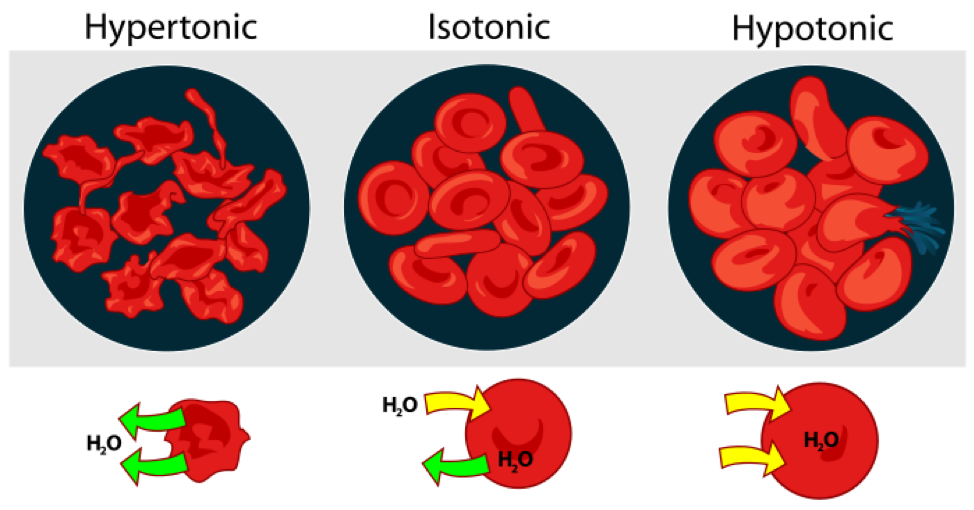
\includegraphics[width=0.7\linewidth]{./figures/exchange/Osmosis_blood}

}

\caption{\href{https://commons.wikimedia.org/wiki/File:Osmotic_pressure_on_blood_cells_diagram.svg}{Osmosis
in red blood cells.}}\label{fig:osmosisb}
\end{figure}

\subsection{Experimental procedures}\label{experimental-procedures-15}

\begin{enumerate}
\def\labelenumi{\arabic{enumi}.}
\tightlist
\item
  Work in groups of three students
\item
  Get three clean slides.
\item
  With a wax pencil, mark the first slide ``5\%'', the
  second ``0.85\%'', and the third ``0\%'' (distilled water).
\item
  Place a drop of the corresponding saline solution (NaCl) and distilled
  water on each slide using a plastic transfer pipette.
\item
  Add a small drop of sheep's blood beside the drop of saline.
\item
  Add a coverslip to each slide immediately, raising and lowering the
  coverslip a couple of times to mix the blood and saline.
\item
  Choose an area where the cells are thinly distributed and observe
  under 400× magnification. The differences are best compared if three
  microscopes are used at once, side by side.
\item
  Compare your observation with the figure shown above.
\end{enumerate}

\section{Turgor and Plasmolysis}\label{turgor-and-plasmolysis}

Osmotic pressure is the main cause of support in many plants. The
osmotic entry of water raises the turgor pressure exerted against the
cell wall, until it equals the osmotic pressure, creating a steady
state. When a plant cell is placed in a solution that is hypertonic
relative to the cytoplasm, water moves out of the cell and the cell
shrinks (Figure \ref{fig:osmosisp}). In doing so, the cell becomes
flaccid. In extreme cases, the cell becomes plasmolyzed - the cell
membrane disengages with the cell wall due to lack of water pressure on
it. When a plant cell is placed in a solution that is hypotonic relative
to the cytoplasm, water moves into the cell and the cell swells to
become turgid. Osmosis is responsible for the ability of plant roots to
draw water from the soil. Plants concentrate solutes in their root cells
by active transport, and water enters the roots by osmosis. Osmosis is
also responsible for controlling the movement of guard cells.

\begin{figure}

{\centering 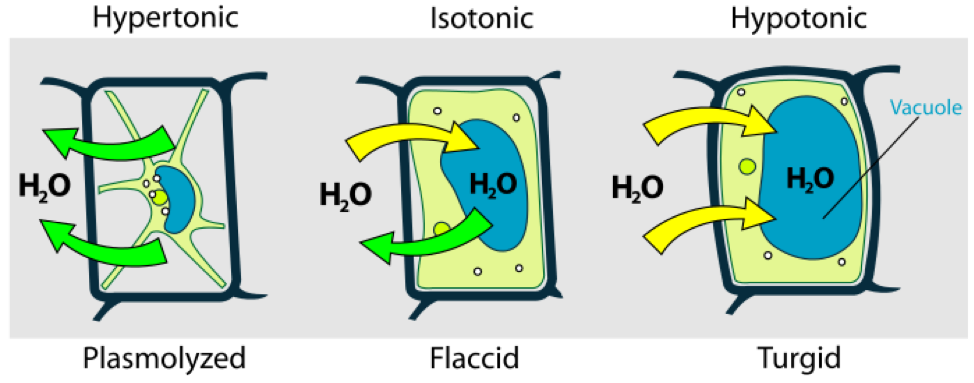
\includegraphics[width=0.7\linewidth]{./figures/exchange/Osmosis_plant}

}

\caption{\href{https://commons.wikimedia.org/wiki/File:Turgor_pressure_on_plant_cells_diagram.svg}{Osmosis
in plant cells.}}\label{fig:osmosisp}
\end{figure}

\subsection{Experimental procedures}\label{experimental-procedures-16}

\begin{enumerate}
\def\labelenumi{\arabic{enumi}.}
\tightlist
\item
  Mount a leaf of Elodea in water on a slide and observe.
\item
  Blot off the water and add salt solution (7\% NaCl) by adding the salt
  at one side of the coverslip and drawing it under by using a paper
  towel to absorb the fluid from the opposite side of the coverslip.
\item
  Let it sit for a minute or two and observe again. The cell contains a
  vacuole, which holds most of the cell's water, similar to a water bag
  inside the cell. Note the clear space forming between the cell wall
  and the cell membrane.
\item
  Rinse the salt solution from the leaf and remount in water.
\item
  Observe periodically for about 5 minutes. How is the cell changing?
\end{enumerate}

\section{Review Questions}\label{review-questions-3}

\begin{enumerate}
\def\labelenumi{\arabic{enumi}.}
\tightlist
\item
  What is and what causes Brownian motion?
\item
  What is the definition of concentration?
\item
  What is a concentration gradient?
\item
  What is diffusion?
\item
  What is a selectively permeable membrane?
\item
  What is osmosis?
\item
  What is osmotic pressure?
\end{enumerate}
